\documentclass[a4paper]{article}

\usepackage{amsmath,tikz}
\usepackage{babel}
\usepackage[utf8]{inputenc}
\usepackage[T1]{fontenc}
\usepackage{tikz}
\usepackage[top = 1cm, bottom = 1cm, left = 1cm, right = 1cm]{geometry}

\begin{document}

\begin{center}
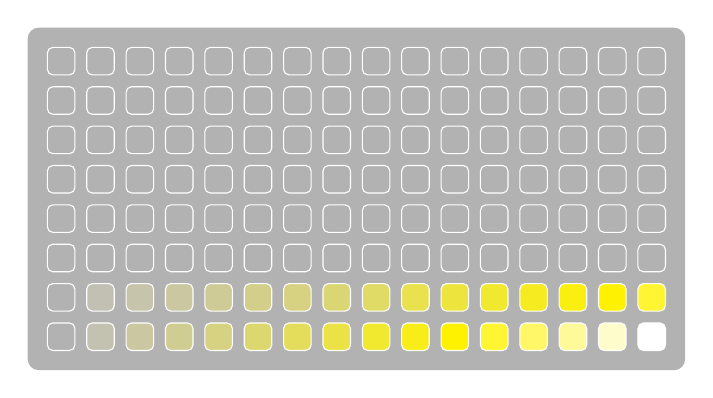
\begin{tikzpicture}[scale = 0.5]
  \fill[black!30!white, rounded corners] (0.3,0.3) rectangle (17,9);

  
  \colorlet{c0}{black!30!white}
  \colorlet{c1}{black!30!white!90!yellow}
  \colorlet{c2}{black!30!white!80!yellow}
  \colorlet{c3}{black!30!white!70!yellow}
  \colorlet{c4}{black!30!white!60!yellow}
  \colorlet{c5}{black!30!white!50!yellow}
  \colorlet{c6}{black!30!white!40!yellow}
  \colorlet{c7}{black!30!white!30!yellow}
  \colorlet{c8}{black!30!white!20!yellow}
  \colorlet{c9}{black!30!white!10!yellow}
  \colorlet{c10}{yellow}
  \colorlet{c11}{yellow!80!white}
  \colorlet{c12}{yellow!60!white}
  \colorlet{c13}{yellow!40!white}
  \colorlet{c14}{yellow!20!white}
  \colorlet{c15}{yellow!0!white}
    

  \colorlet{d0}{black!30!white}
  \colorlet{d1}{black!30!white!93!yellow}
  \colorlet{d2}{black!30!white!86!yellow}
  \colorlet{d3}{black!30!white!80!yellow}
  \colorlet{d4}{black!30!white!73!yellow}
  \colorlet{d5}{black!30!white!66!yellow}
  \colorlet{d6}{black!30!white!60!yellow}
  \colorlet{d7}{black!30!white!53!yellow}
  \colorlet{d8}{black!30!white!46!yellow}
  \colorlet{d9}{black!30!white!33!yellow}
  \colorlet{d10}{black!30!white!26!yellow}
  \colorlet{d11}{black!30!white!20!yellow}
  \colorlet{d12}{black!30!white!13!yellow}
  \colorlet{d13}{black!30!white!6!yellow}
  \colorlet{d14}{yellow}
  \colorlet{d15}{yellow!80!white}



  
  \foreach \x \y \z in {
    1/1/c0,
    2/1/c1,
    3/1/c2,
    4/1/c3,
    5/1/c4,
    6/1/c5,
    7/1/c6,
    8/1/c7,
    9/1/c8,
    10/1/c9,
    11/1/c10,
    12/1/c11,
    13/1/c12,
    14/1/c13,
    15/1/c14,
    16/1/c15,
    1/2/d0,
    2/2/d1,
    3/2/d2,
    4/2/d3,
    5/2/d4,
    6/2/d5,
    7/2/d6,
    8/2/d7,
    9/2/d8,
    10/2/d9,
    11/2/d10,
    12/2/d11,
    13/2/d12,
    14/2/d13,
    15/2/d14,
    16/2/d15}{
      \fill[fill = \z, rounded corners=2pt] (\x-0.2,\y - 0.2) rectangle (\x + .5, \y + .5) {};
    }
    
    

 % draw after filling
  \foreach \x in {1,...,16}
    \foreach \y in {1,...,8}
    {\draw[draw = white, rounded corners=2pt] (\x-0.2,\y - 0.2) rectangle (\x + .5, \y + .5) {};
    }
    
      
\end{tikzpicture}
\end{center}

\end{document}

%%% Local Variables:
%%% mode: latex
%%% TeX-master: t
%%% End:
